% !TeX program = xelatex
\documentclass{beamer}

% Theme settings
\usetheme{Madrid}
\usecolortheme{default}

% Font settings
\usepackage{xeCJK}
\setCJKmainfont{PingFang TC}  % For any Chinese characters
\setCJKsansfont{PingFang TC}
\setCJKmonofont{PingFang TC}

% Other packages
\usepackage{graphicx}
\usepackage{amsmath}
\usepackage{amssymb}
\usepackage{float}  % For better image placement

% Title information
\title{Digital Logic and Minecraft Implementation}
\author{Author: Jian Wei Heng, Xu Shun Jie, Lu Yong Han}
\institute{Fu Jen Catholic University}
\date{\today}

\begin{document}

% Title page
\begin{frame}
    \titlepage
\end{frame}

% Table of contents
\begin{frame}{Table of Contents}
    \tableofcontents
\end{frame}

% First chapter
\section{Digital Logic Basics}
\begin{frame}{Basic Concepts of Digital Logic}
    \begin{itemize}
        \item Digital logic uses binary system (0 and 1)
        \item 0 represents low voltage (Low)
        \item 1 represents high voltage (High)
        \item These states can be implemented through circuits
    \end{itemize}
    \begin{figure}[ht]
        \centering
        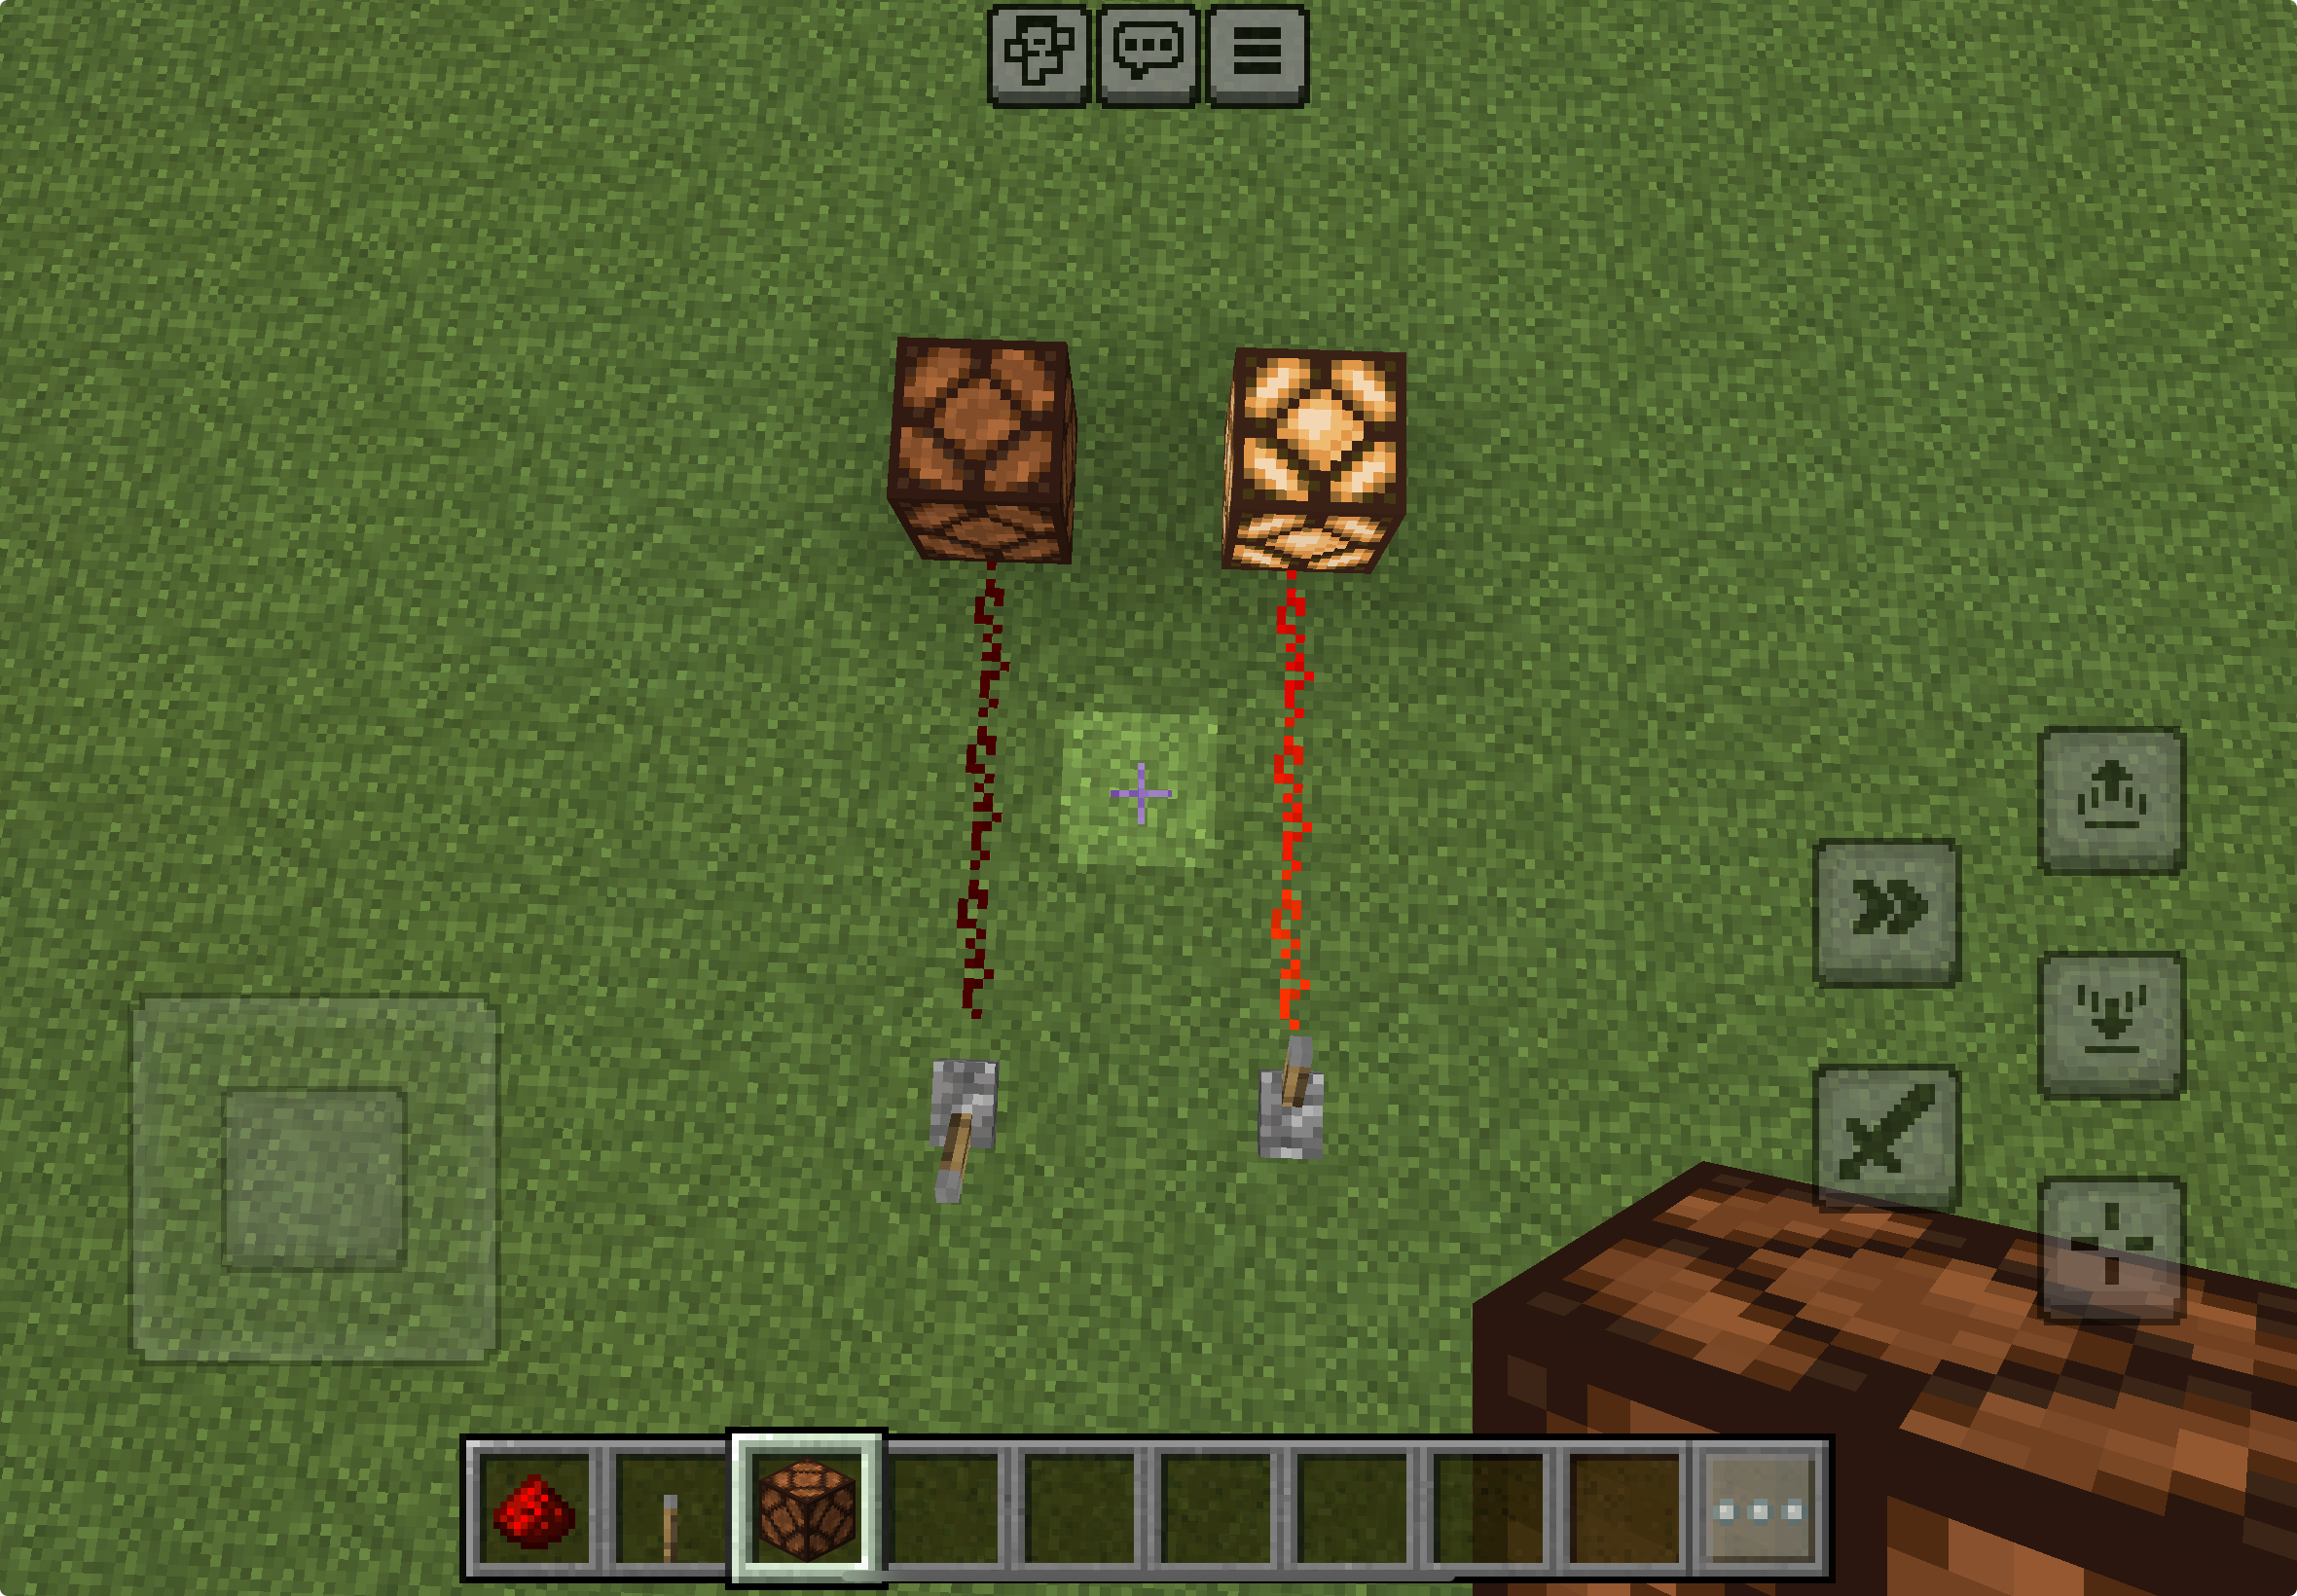
\includegraphics[width=0.6\textwidth]{images/zero_and_one_gate.png}
        \caption{Example of 0 and 1 in Minecraft Redstone Circuit}
    \end{figure}
\end{frame}

\begin{frame}{Basic Logic Gates}
    \begin{itemize}
        \item AND Gate: Output is 1 only when both inputs are 1
        \item OR Gate: Output is 1 when any input is 1
        \item NOT Gate: Output is opposite of input
        \item NAND Gate: AND Gate output inverted
        \item NOR Gate: OR Gate output inverted
    \end{itemize}
\end{frame}

\begin{frame}{AND Gate in Minecraft}
    \begin{itemize}
        \item The AND gate outputs 1 only when both inputs are 1.
        \item In Minecraft, you can use redstone components to build an AND gate.
        \item Below are examples of different input combinations and their outputs:
    \end{itemize}
    \begin{figure}[ht]
        \centering
        \begin{minipage}{0.32\textwidth}
            \centering
            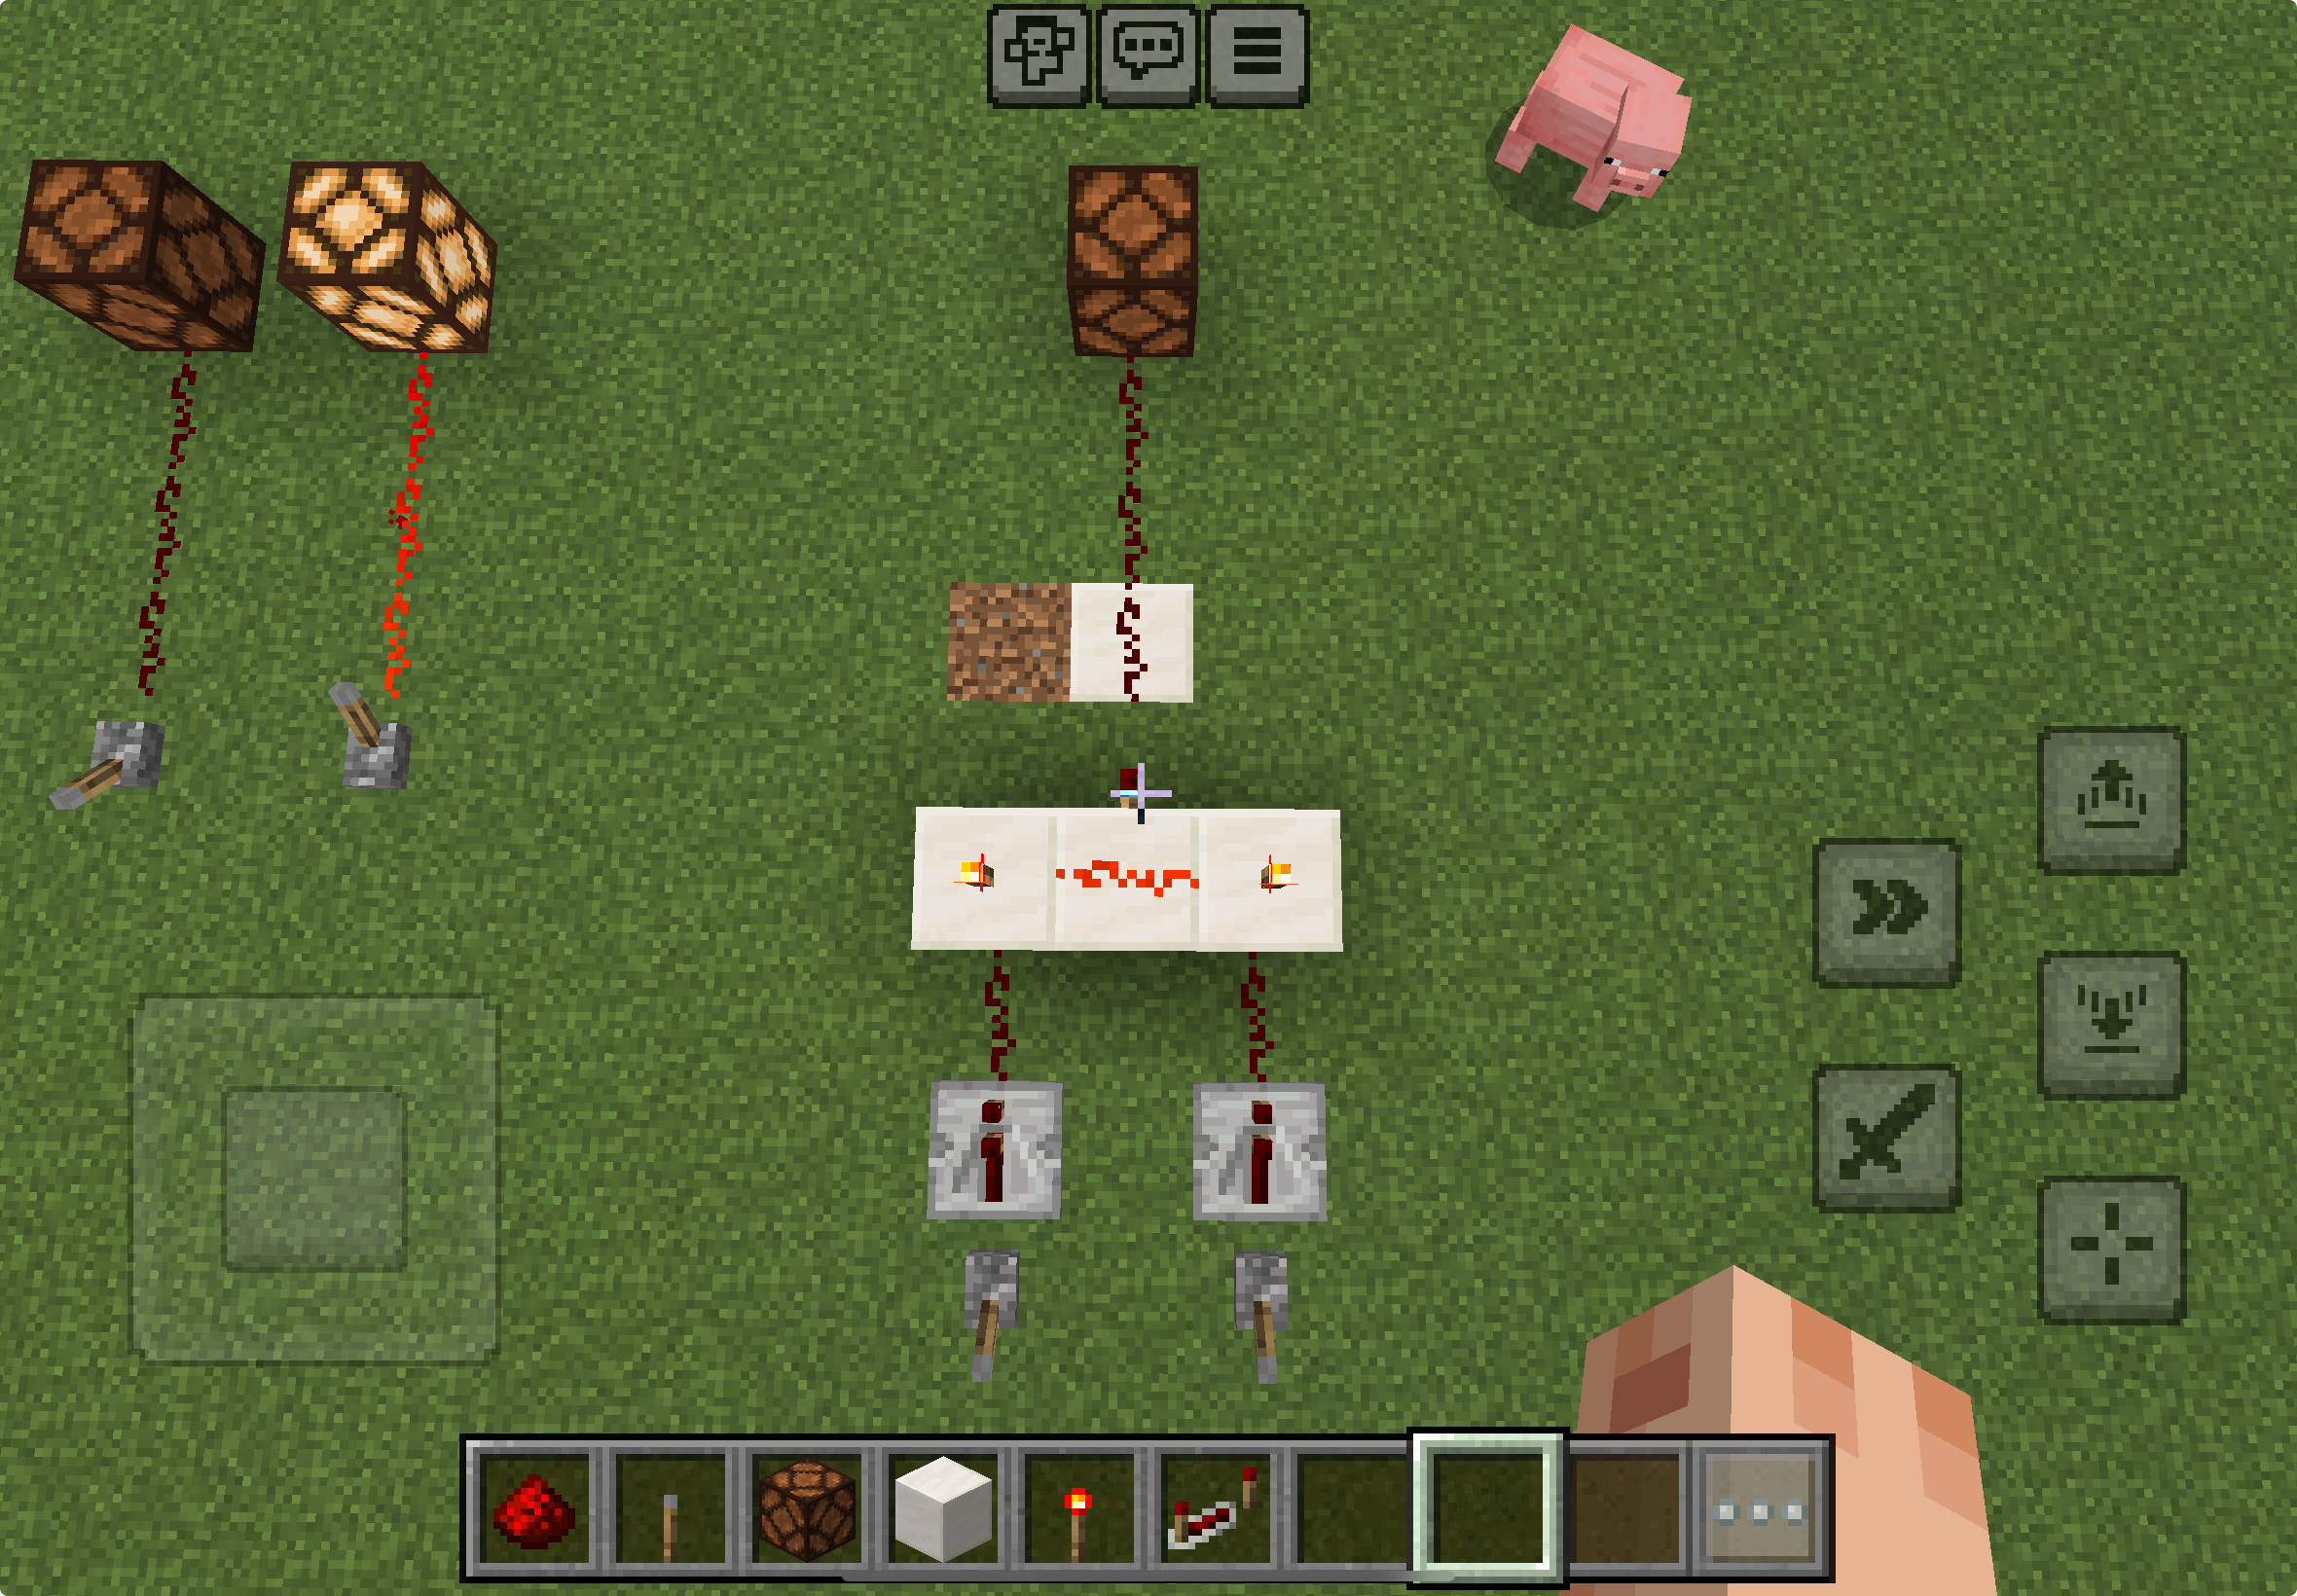
\includegraphics[width=\textwidth]{images/andgate_00.png}\\
            \small Input: 0, 0
        \end{minipage}
        \begin{minipage}{0.32\textwidth}
            \centering
            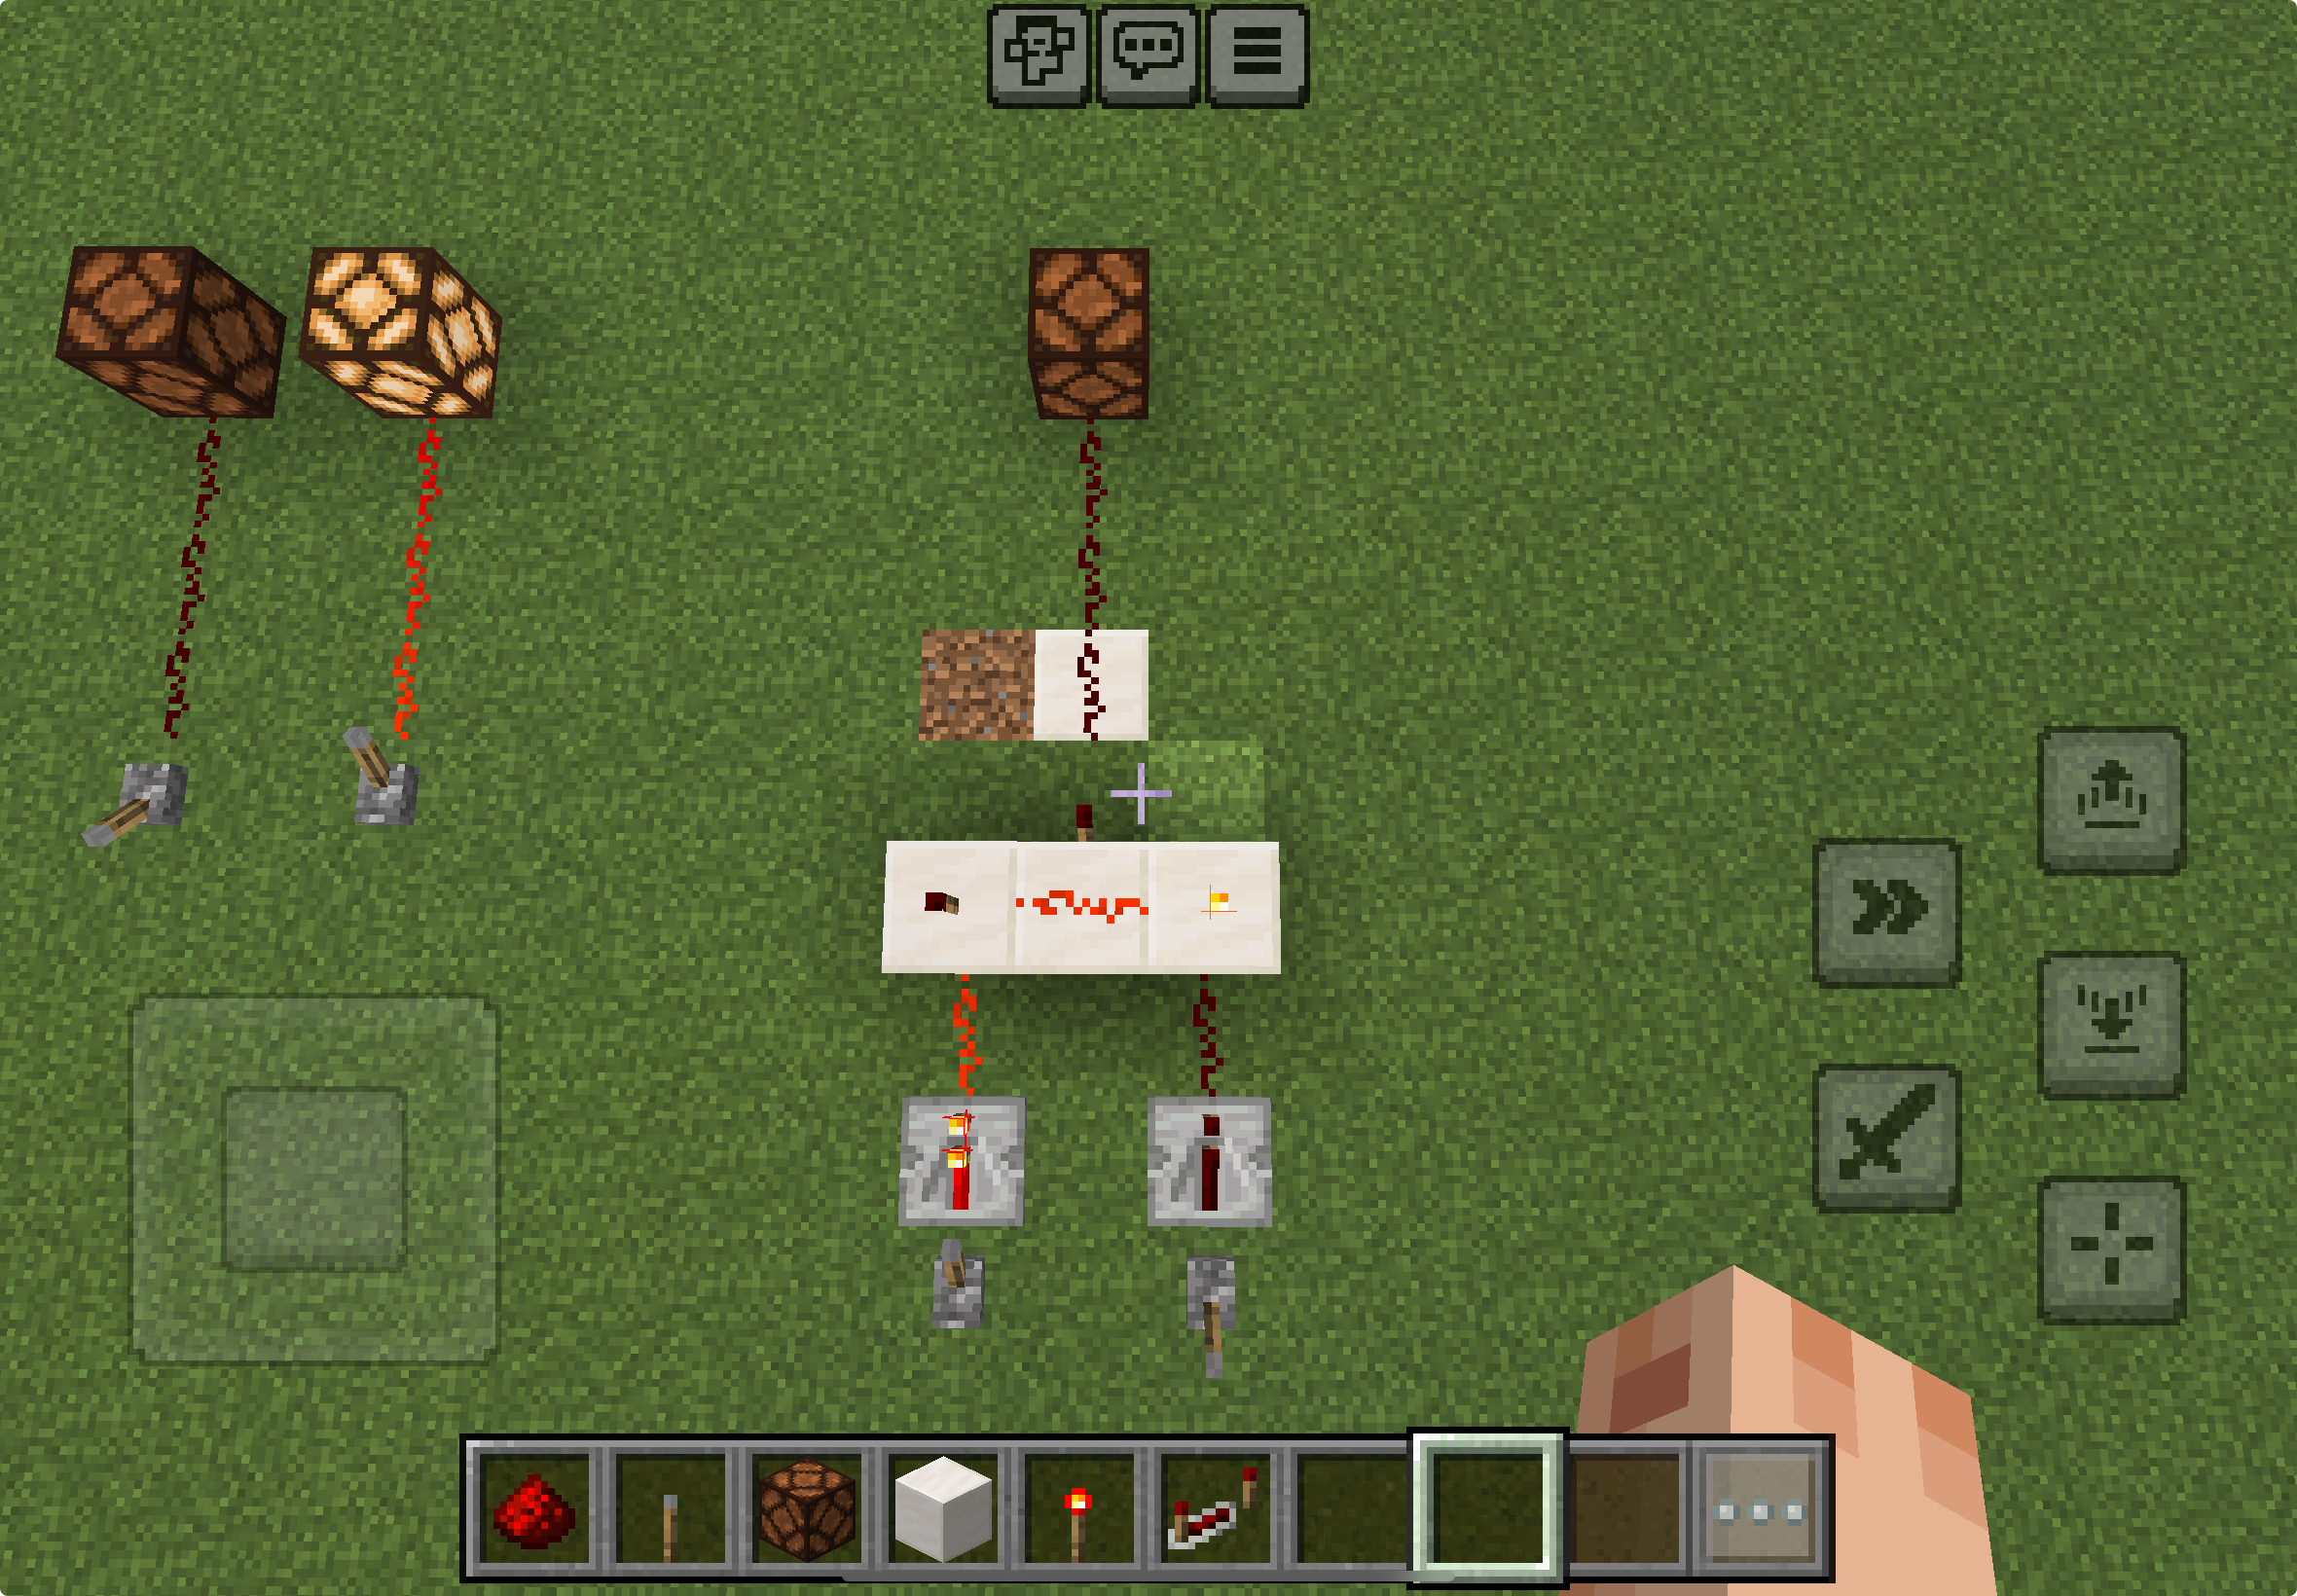
\includegraphics[width=\textwidth]{images/andgate_01.png}\\
            \small Input: 0, 1
        \end{minipage}
        \begin{minipage}{0.32\textwidth}
            \centering
            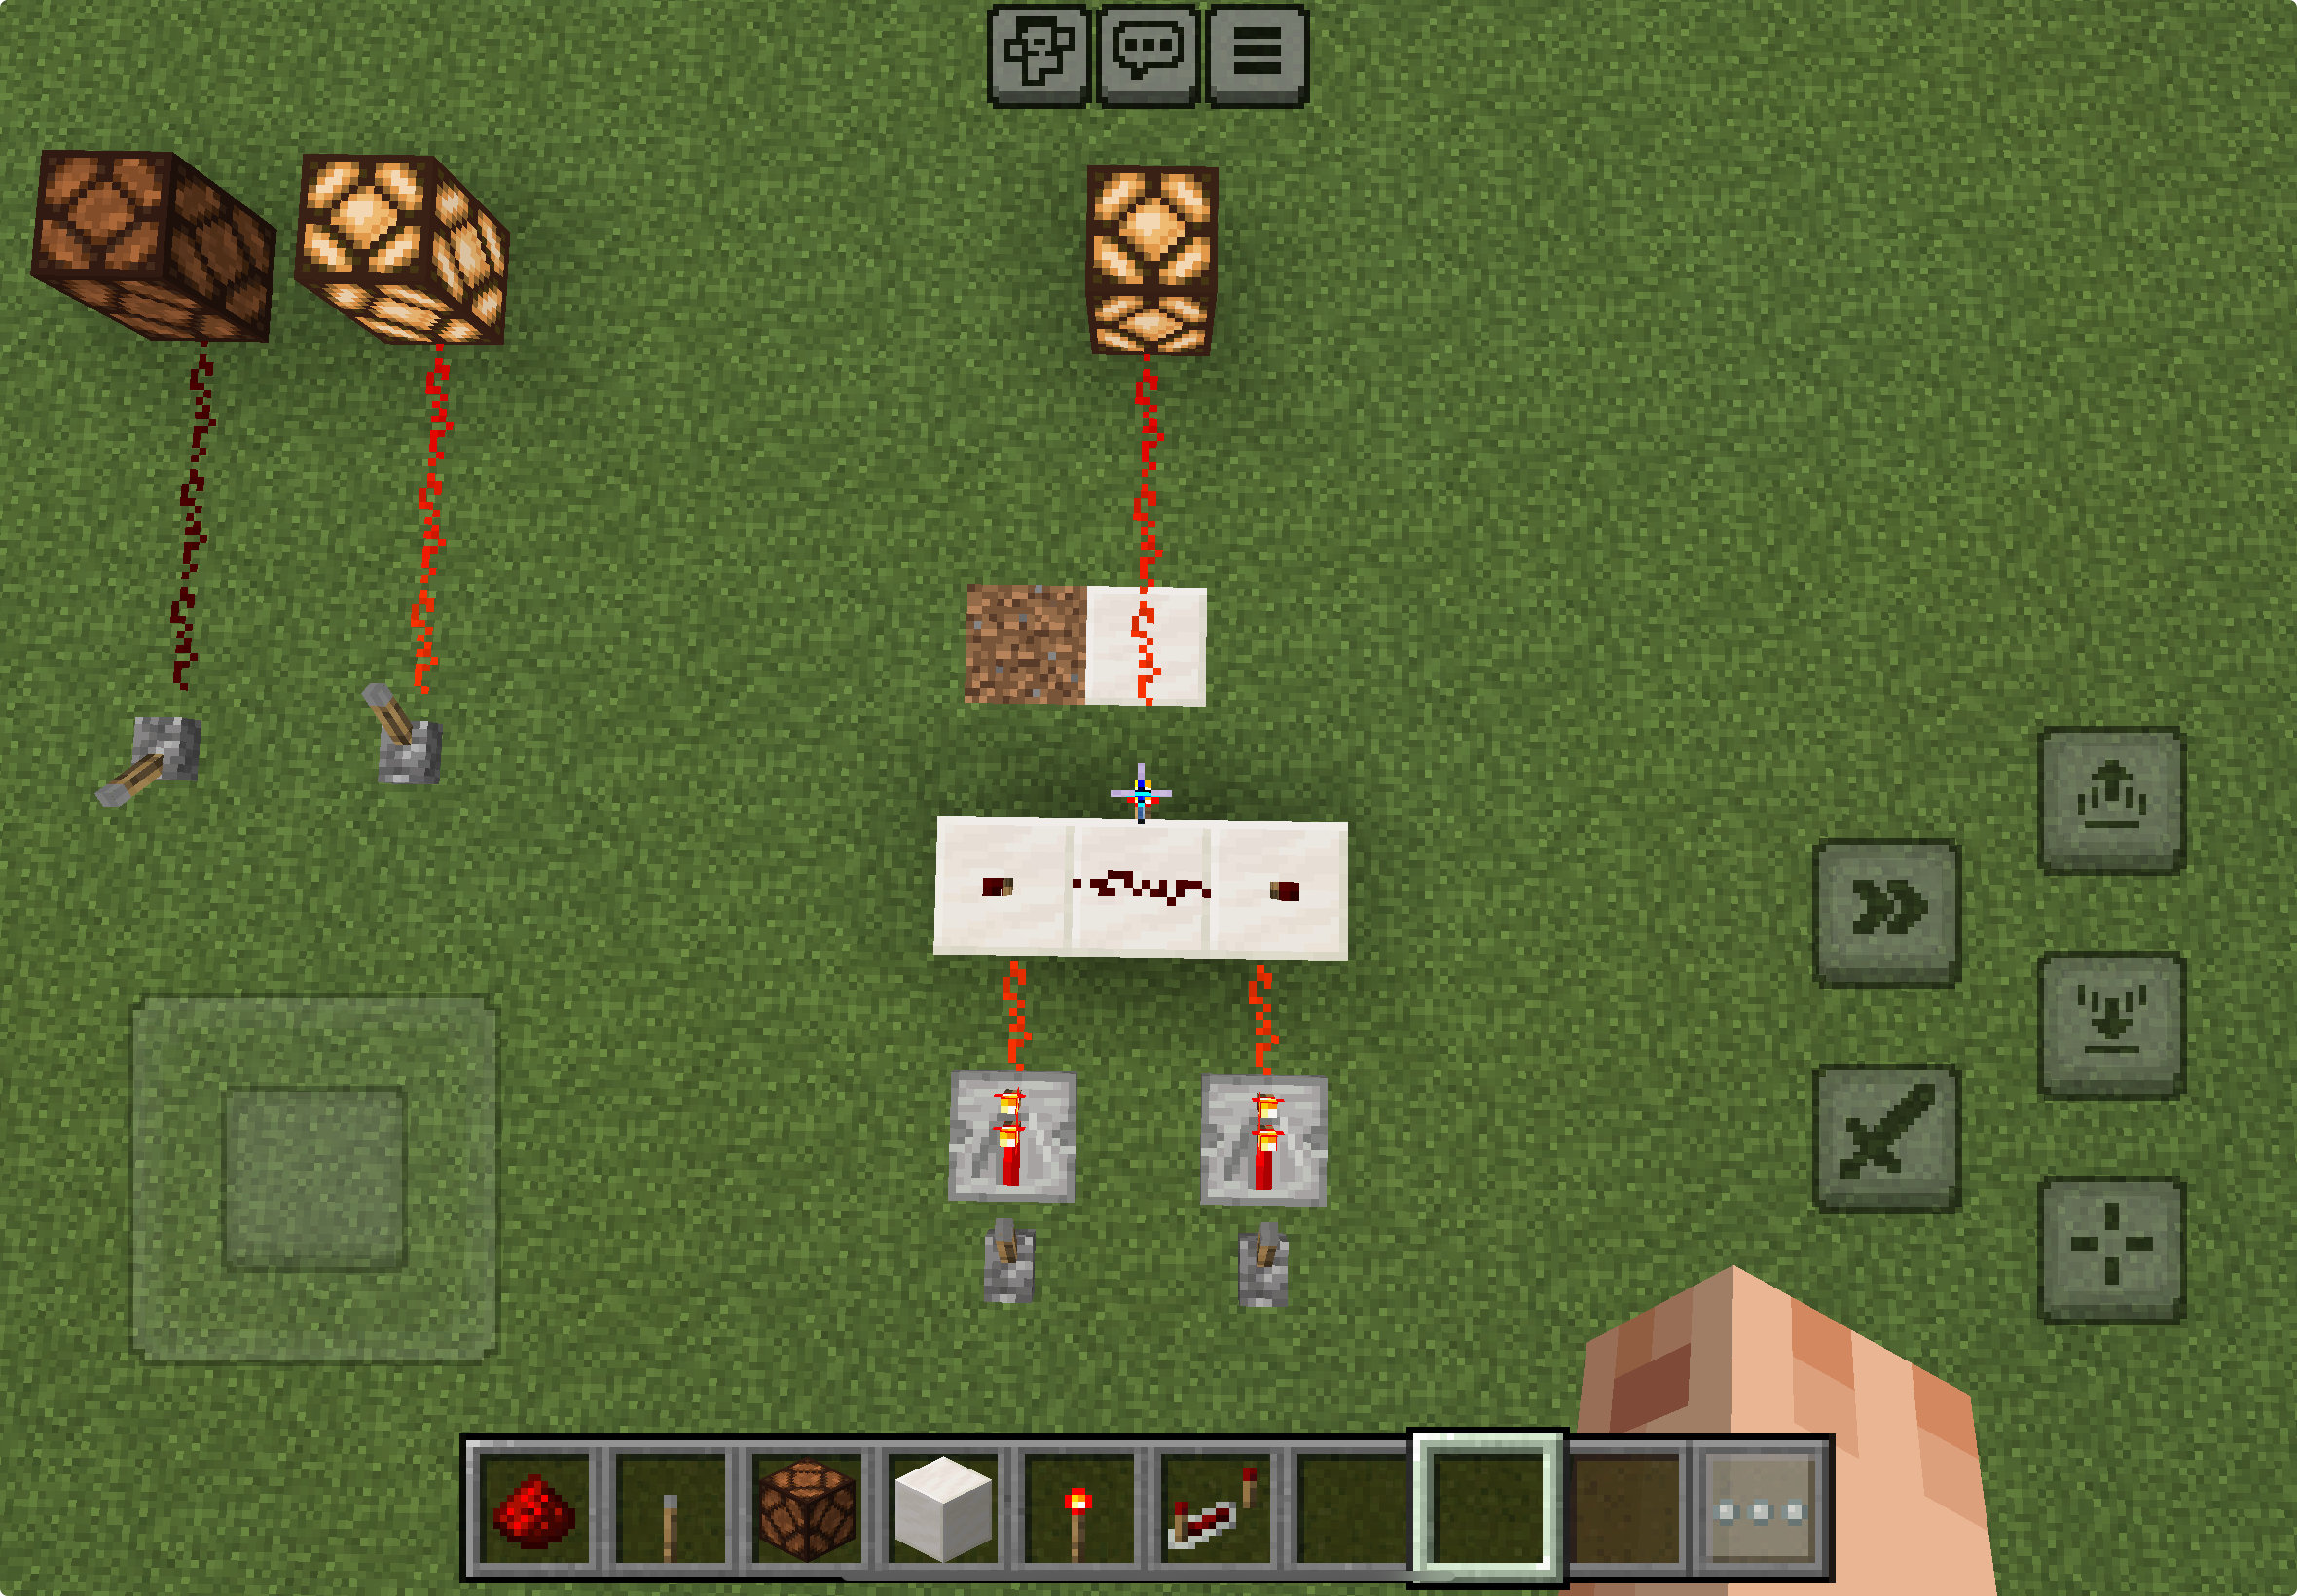
\includegraphics[width=\textwidth]{images/andgate_11.png}\\
            \small Input: 1, 1
        \end{minipage}
        \caption{AND Gate in Minecraft: Different Input Combinations}
    \end{figure}
\end{frame}

\begin{frame}{Logic Gate Truth Tables}
    \begin{block}{AND Gate}
        \begin{tabular}{|c|c|c|}
            \hline
            Input A & Input B & Output \\
            \hline
            0 & 0 & 0 \\
            0 & 1 & 0 \\
            1 & 0 & 0 \\
            1 & 1 & 1 \\
            \hline
        \end{tabular}
    \end{block}
\end{frame}

\begin{frame}{Logic Gate Truth Tables}
    \begin{block}{OR Gate}
        \begin{tabular}{|c|c|c|}
            \hline
            Input A & Input B & Output \\
            \hline
            0 & 0 & 0 \\
            0 & 1 & 1 \\
            1 & 0 & 1 \\
            1 & 1 & 1 \\
            \hline
        \end{tabular}
    \end{block}
\end{frame}

\begin{frame}{Logic Gate Truth Tables}
    \begin{block}{NOT Gate}
        \begin{tabular}{|c|c|}
            \hline
            Input & Output \\
            \hline
            0 & 1 \\
            1 & 0 \\
            \hline
        \end{tabular}
    \end{block}
\end{frame}

% Second chapter
\section{Minecraft Implementation}
\begin{frame}{Redstone System in Minecraft}
    \begin{itemize}
        \item Redstone Dust: Transmits signals
        \item Redstone Torch: Generates signals
        \item Redstone Repeater: Delays and amplifies signals
        \item Redstone Comparator: Compares signal strengths
    \end{itemize}
\end{frame}

\begin{frame}{Logic Gate Implementation in Minecraft}
    \begin{block}{Basic Logic Gates}
        \begin{itemize}
            \item NOT Gate: Using redstone torch
            \item AND Gate: Using two redstone torches in series
            \item OR Gate: Using two redstone torches in parallel
        \end{itemize}
    \end{block}
    
    \begin{alertblock}{Note}
        In Minecraft, the on/off state of redstone torches is opposite to the logic gate input/output
    \end{alertblock}
\end{frame}

\begin{frame}{Practical Applications in Minecraft}
    \begin{itemize}
        \item Automatic Door Systems
        \item Trap Mechanisms
        \item Automatic Farms
        \item Item Sorting Systems
    \end{itemize}
\end{frame}

% End page
\begin{frame}{Thank You}
    \centering
    Thank you for listening!
\end{frame}

\end{document}
